\documentclass{report}
\usepackage[fontsize=13pt]{scrextend}

\usepackage{my_lab}

\begin{document}

\graphicspath{{figures}}

\MiptLabTitle{4.5.2}{}

\begin{document}

\textbf{Цель работы}: исследовать зависимость видности интерфереционной картины
от разности хода интерферирующих лучей и от их поляризации.

\textbf{В работе используются}: He-Ne лазер, интерферометр Майкельсона с
подвижным зеркалом, фотодиод с усилителем, осциллограф С1-76, поляроид,
линейка.

\section*{Теория}

\subsection*{Гелий-неоновый лазер}

Лазер представляет собой интерферометр Фабри-Перо -- газовую трубку с двумя
параллельными зеркалами по обе стороны. В лазере длиной $L$ для излучения вдоль
о,и для резонансных частот выполняется

\begin{equation}
f_m = \dv{c}{\lambda_m} = \dv{mc}{2L}.
\end{equation}

Условие генерации может выполняться для сразу нескольких колебаний с частостами
$f_m$, разположенными в диапазоне генерации $2\Delta F$. В этом случае
генерируется несколько волн -- \textit{мод} -- межмодовое расстояние для
которых

\begin{equation}
\Delta \nu = f_{m+1} - f_m = \dv{c}{2L}.
\end{equation}

Число мод можно оценить как

\begin{equation}
N \approx 1 + \dv{2\Delta F}{\Delta \nu}.
\end{equation}

\subsection*{Видимость}

Видимость интерфереционной картины -- параметр, определяемый формулой

\begin{equation}
\gamma = \dv{I_{max} - I_{min}}{I_{max} + I_{min}},
\end{equation}

где $I_{max}$, $I_{min}$ -- максимальная и минимальная интенсивности света
интерфереционной картины вблизи выбранной точки. Разобьём его на произведение
функций параметров установки
$$
\gamma = \gamma_1 \gamma_2 \gamma_3.
$$
Здесь $\gamma_1$ отвечает за соотношение интенсивности интерферирующих волн:
\begin{equation}
\gamma_1 = \dv{2\sqrt{\delta}}{1+\delta},
\end{equation}

где $\delta = \frac{B_m^2}{A_m^2}$, $A_m$ и $B_m$ -- амплитуды волн. Параметр
$\delta$ определяется устройством разделения волн.\\
Функция $\gamma_2$ отвечает за влияние разности хода и спектрального состава волн,

\begin{wrapfigure}{r}{0.4\textwidth}
\begin{center}
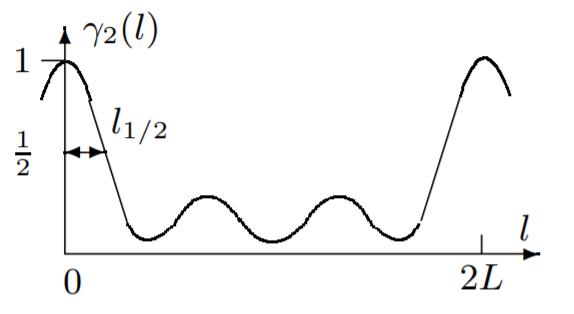
\includegraphics[width = 0.4\textwidth]{1.png}
\vspace{-20pt}
\end{center}
\caption{Зависимость $\gamma_2 = \gamma_2(l)$.}
\end{wrapfigure}
$$
\gamma_2 = \dv{\sum\limits_n A^2_n \cos \frac{2\pi \Delta \nu n l}{c}}{\sum\limits_n A_n^2},
$$
где $l$ -- разность хода, $\Delta \nu$ -- спектральный состав излучения,
$A_n^2$ -- интенсивности мод. В непрерывном пределе получим
$$
\gamma_2 = e^{-\left(\frac{\pi \Delta F l}{c}\right)^2}
$$
-- для гауссова линии излучения с полушириной $\Delta F$ получили гауссову
зависимость $\gamma_2 = \gamma_2(l)$ с полушириной

\begin{equation}
l_{1/2} = \dv{c}{\pi \Delta F}\sqrt{\ln 2} \approx \dv{0.26 c}{\Delta F}.
\end{equation}

Последняя функция $\gamma_3$ отвечает за разность в поляризации.
Если $\alpha$ -- угол между плоскостями поляризаций волн, то

\begin{equation}
\gamma_3 = |\cos \alpha|.
\end{equation}

\subsection*{Установка}

\begin{figure}[h]
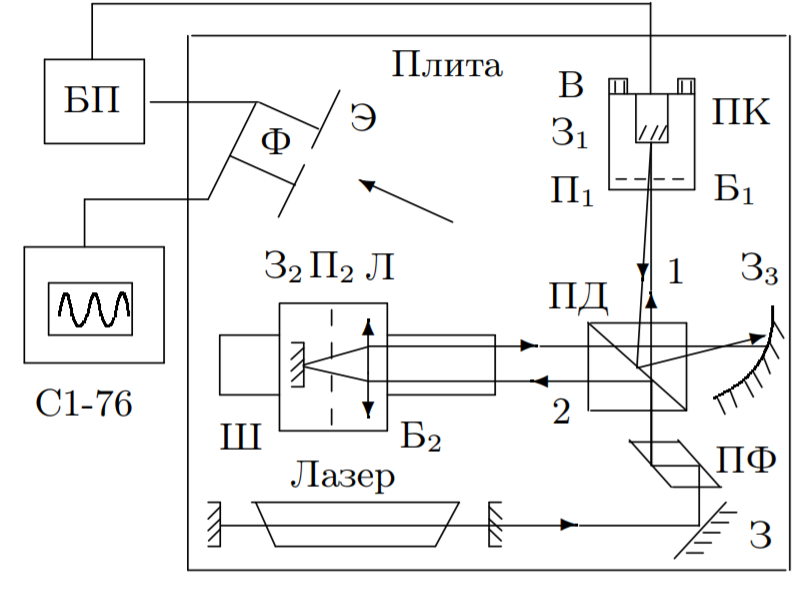
\includegraphics[scale=0.55]{2.png}
\centering
\caption{Схема установки.}
\end{figure}

В работе используется интерферометр Майкельсона (Рис. 2). Луч лазера,
отражённый от зеркала З и прошедший через параллелепипед Френеля (ПФ), делится
делительной призмой ДП на два луча. Первый проходит блок $\text{Б}_1$ с
поляроидом $\text{П}_1$ и зеркалом $\text{З}_1$, прикленным к пьезокерамике,
которая может совершать малые колебания вдоль луча, с возможность изменения
угла наклона зеркала. Второй проходит блок $\text{Б}_2$ с линзой Л, поляроидом
$\text{П}_2$ и зеркалом $\text{З}_2$ в фокальной плоскости линзы, чтобы
выходящий луч, в отличие от первого, был параллелен входящему. Оба луча,
проходя ДП, попадают на сферическое зеркало $\text{З}_3$ и интерферируют на
экране. Интенсивность света считывается фотодиодом на осциллограф через щель,
параллельную интерфереционным полосам, в центре экрана. На экране осциллографа
наблюдаются колебания с изменяющимся периодом, так как на пьезокерамику
подаются напряжение, из-за чего её длина колеблется.

\begin{wrapfigure}{l}{0.4\textwidth}
\begin{center}
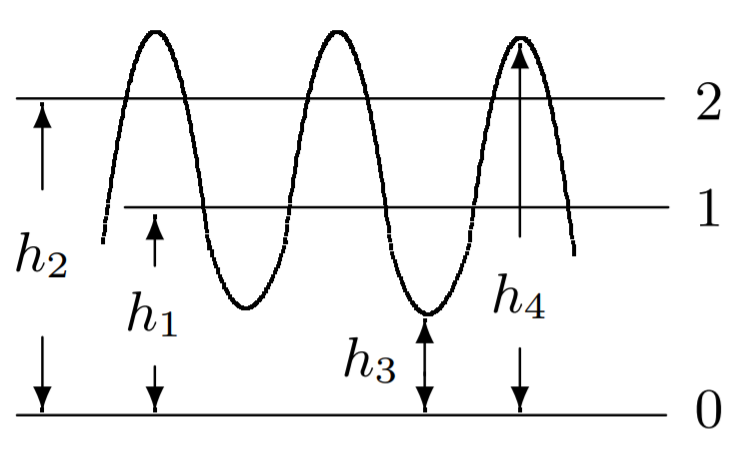
\includegraphics[width = 0.4\textwidth]{3.png}
\vspace{-40pt}
\end{center}
\caption{Осциллограмма сигналов фотодиода.}
\end{wrapfigure}

По картине на экране осциллографа можно определить параметры видимости по следующим формулам:

\begin{equation}
\delta = \dv{h_1}{h_2},
\end{equation}
\begin{equation}
\gamma = \dv{h_4 - h_3}{h_4 + h_3},
\end{equation}

Здесь 0 -- уровень при отсутствии лучей, 1 и 2 -- при закрытии одного из них.
Используя $\delta$, можно рассчитать $\gamma_1$ по формуле (5).\\
При условии одинаковой поляризации лучей ($\alpha = 0$),
\begin{equation}
\gamma_2 = \dv{\gamma}{\gamma_1}.
\end{equation}

Если же разность хода отсутствует ($l = 0$), то
\begin{equation}
\gamma_3 = \dv{\gamma}{\gamma_1}.
\end{equation}

\end{document}
